%! TEX program = pdflatex

\documentclass[oneside,solution]{karazin-complan-assign}

\usepackage[utf8]{inputenc}
\usepackage[english,ukrainian]{babel}

\usepackage{mathtools}

\let\Im\relax
\DeclareMathOperator{\Im}{Im}
\let\Re\relax
\DeclareMathOperator{\Re}{Re}

\usetikzlibrary{decorations.markings,positioning}

\providecommand{\poles}{
  \node (poles) at (2.5,1.5) {poles of $h(p_0)$};
  \draw[fill]
  (1.5,3) coordinate [circle,fill,inner sep=1pt,label=right:$p_1$] (p1)
  (2,-2) coordinate [circle,fill,inner sep=1pt,label=below:$p_2$] (p2)
  (-3,1) coordinate [circle,fill,inner sep=1pt,label=above:$p_3$] (p3)
  (-2,-1.5) coordinate [circle,fill,inner sep=1pt,label=above:$p_4$] (p4);
  \draw[ultra thin,gray] (poles) -- (p1) (poles) -- (p2) (poles.west) -- (p3) (poles) -- (p4);
}

\def\xr{3.5}
\def\yr{3}


\title{Домашня робота}
\author{Захаров Дмитро}
\studentID{МП-31}
\instructor{Гиря Н.П.}
\date{\today}
\duedate{23:59 12 травня, 2024}
\assignno{5}
\semester{Весняний семестр 2024}
\mainproblem{Відображення \#2. Варіант 5}

\begin{document}

\maketitle

% \startsolution[print]

\problem{Лінійно-дробове відображення}

\hspace{20px}\textbf{Умова.} Знайти образ області при заданому відображенні:
\begin{equation}
    \mathcal{D} = \{z \in \mathbb{C}: |z|<1 \wedge \text{Im}(z) > 0\}, \; \omega(z) = \frac{1}{z}
\end{equation}

\textbf{Розв'язок.} Наша область $\mathcal{D}$ -- верхня одинична півкуля (або кругова луночка). Вона обмежена дугою $\gamma$ та відрізком $[-1,1]$ ($\partial\mathcal{D} = \gamma \cup [-1,1]$). Отже, для того щоб визначити образ, потрібно дослідити, як змінюються дуга та відрізок під дією $\omega$.

\textbf{Відрізок.} Маємо дійсні числа $x$ від $-1$ до $1$, вони перетворяться на дійсну множину $\mathbb{R} \setminus (-1,1)$ під дією відображення $x \mapsto \frac{1}{x}$.

\textbf{Дуга.} Тут ситуація цікавіша. Особлива точка $z=0$ не лежить на $\gamma$, тому дуга перетвориться на іншу дугу. Оскільки $\forall z \in \gamma: |\omega(z)| = \frac{1}{|z|} = 1$, то знову ж таки маємо дугу на одиничній кулі. Причому, $\omega(e^{i\varphi}) = e^{-i\varphi}$, тобто $\omega$ просто діє як оператор спряження $z \mapsto \overline{z}$ -- таким чином, ми отримуємо нижню півкулю. 

Отже, наша границя образу поки виглядає приблизно як це показано на Рисунку \ref{fig:1(1)}. Залишилося визначитися з тим, де знаходиться сама область. Для цього підставимо якусь точку з області $\mathcal{D}$, наприклад $z=\frac{i}{2}$. Тоді $\omega(\frac{i}{2}) = \frac{2}{i} = -2i$ -- лежить у нижній напівплощині. Отже, замальовувати ми маємо так, як це показано на Рисунку \ref{fig:1(2)}.

\begin{figure}
    \centering
    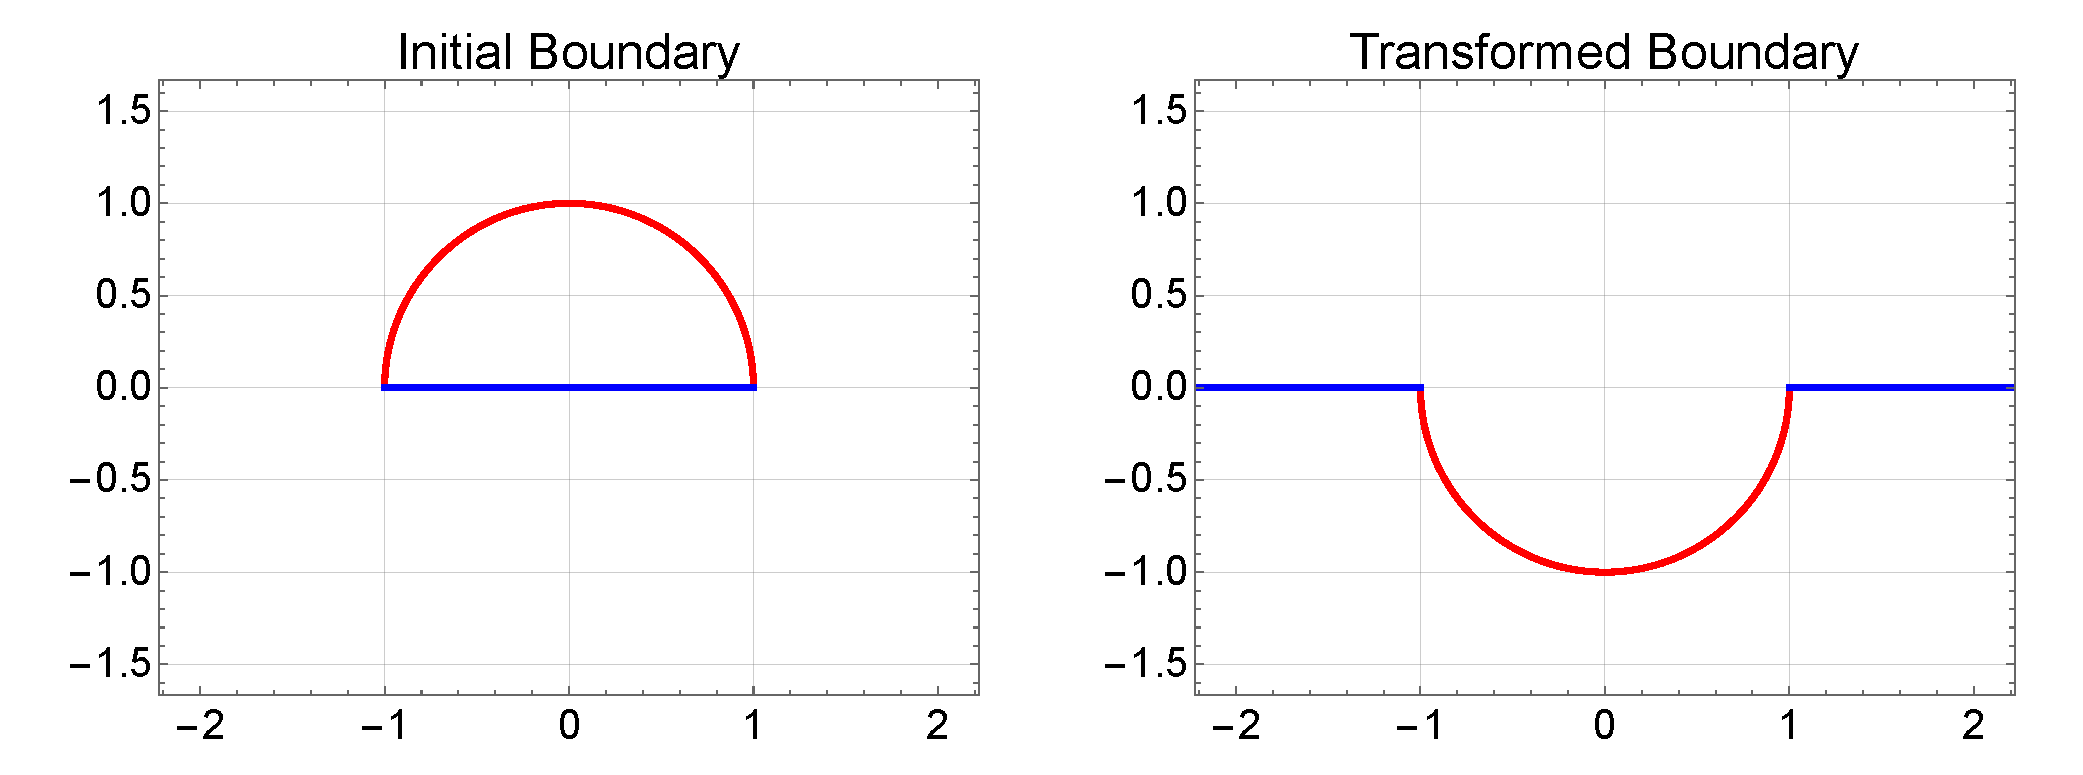
\includegraphics[width=0.85\textwidth]{images/hw_5/problem_1(1).pdf}
    \caption{Границя $\partial\omega(\mathcal{D})$. \textcolor{red}{Червоним} показано $\omega(\gamma)$, а \textcolor{blue}{синім} $\omega([-1,1])$.}
    \label{fig:1(1)}
\end{figure}

\begin{figure}
    \centering
    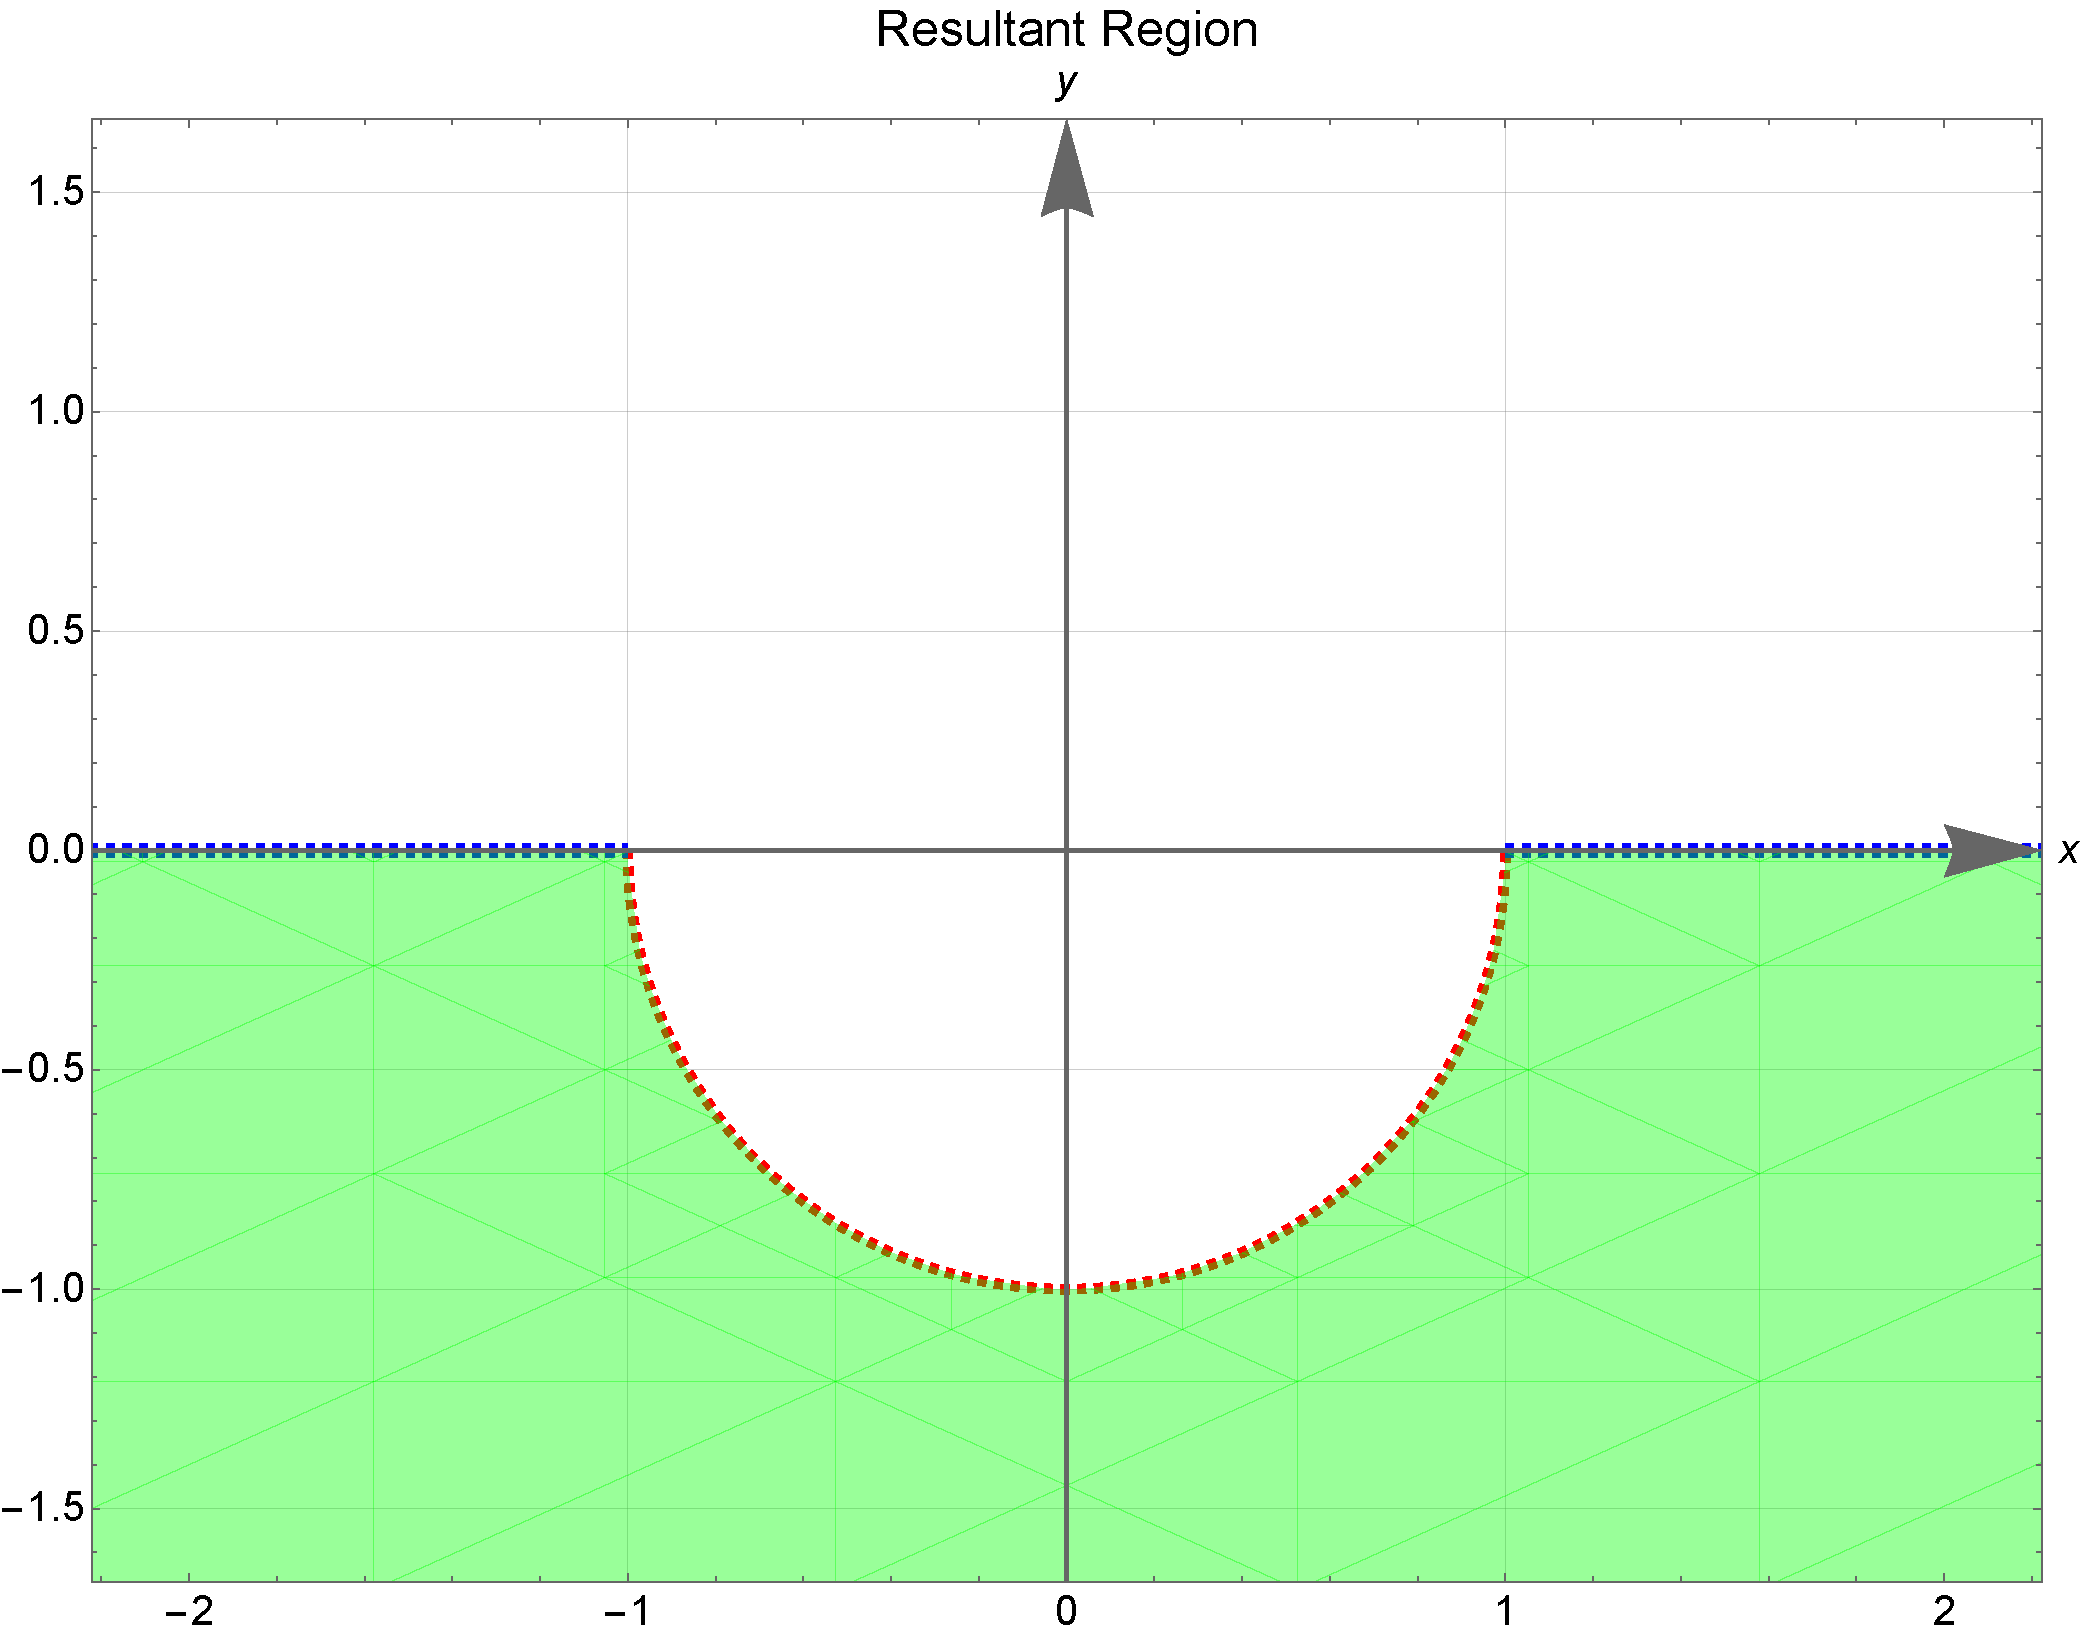
\includegraphics[width=0.7\textwidth]{images/hw_5/problem_1(2).pdf}
    \caption{\textcolor{ForestGreen}{Зеленим} показано шуканий образ $\omega(\mathcal{D})$.}
    \label{fig:1(2)}
\end{figure}

\problem{Експоненційне відображення}

\hspace{20px}\textbf{Умова.} Знайти образ області при заданому відображенні:
\begin{equation}
    \mathcal{D} = \{z \in \mathbb{C}: -1 < \text{Re}(z) < 0, -1 < \text{Im}(z)< 0\}, \; \omega(z) = e^z
\end{equation}

\textbf{Розв'язок.} Маємо квадрат $[-1,0] \times [-1,0]$ на комплексній площині. Тому, розіб'ємо $\partial\mathcal{D} = \gamma_X^+ \cup \gamma_Y^+ \cup \gamma_X^- \cup \gamma_Y^-$, де $\gamma_X^+,\gamma_X^-$ -- права і ліва вертикальні сторони квадрату, відповідно, а $\gamma_Y^+,\gamma_Y^-$ -- верхня і нижня сторони. Розглянемо кожну сторону окремо.

\textcolor{red}{\textbf{Сторона $\boldsymbol{\gamma_X^+}$.}} Можемо параметризувати її як $z(t) = it$ для $t \in [-1,0]$, тому $\omega(z(t)) = e^{it}$ -- дає дугу кола від $e^{-i}=\cos 1 - i\sin 1$ до $1$ з величиною кута в один радіан.

\textcolor{blue}{\textbf{Сторона $\boldsymbol{\gamma_Y^+}$.}} Маємо параметризацію відрізку $z(t) = t$ для $t \in [-1,0] \xleftarrow[]{}$ (ліворуч). Відображення має вигляд $\omega(z(t))=e^t$, а тому образом буде дійсний відрізок від $1$ до $\frac{1}{e}$.

\textcolor{ForestGreen}{\textbf{Сторона $\boldsymbol{\gamma_X^-}$.}} Параметризуємо $z(t) = -1 + it$ для $t \in [-1,0] \xleftarrow[]{}$ (вниз). Тоді відображення $\omega(z(t))=e^{-1+it} = \frac{1}{e} \cdot e^{it}$ -- маємо коло радіусу $\frac{1}{e}$ від точки $\frac{1}{e} \cdot e^{-i}=\frac{\cos 1}{e} - \frac{\sin 1}{e}$ до $\frac{1}{e}$. 

\textcolor{purple}{\textbf{Сторона $\boldsymbol{\gamma_Y^-}$.}} Параметризуємо $z(t) = t - i$ для $t \in [-1,0]$ (праворуч). Тоді відображення $\omega(z(t))=e^{t-i} = e^t(\cos 1 - i \sin 1)$ -- маємо відрізок від $\frac{\cos 1}{e} - \frac{i \sin 1}{e}$ до $\cos 1 - i \sin 1$.

Звучить це достатньо неінтуїтивно, тому намалюємо: маємо Рисунок \ref{fig:2(1)}. Залишилося обрати, де замальовувати область. Легше взяти точку за областю: наприклад, нехай $z_0=100$. Тоді, $\omega(z_0)=e^{100}$ -- точка явно опинилася за областю. Це означає, що точки всередині області залишаються в області, а тому замальовувати треба \textbf{всередині}. Результат зображено на Рисунку \ref{fig:2(2)}.

\begin{figure}
    \centering
    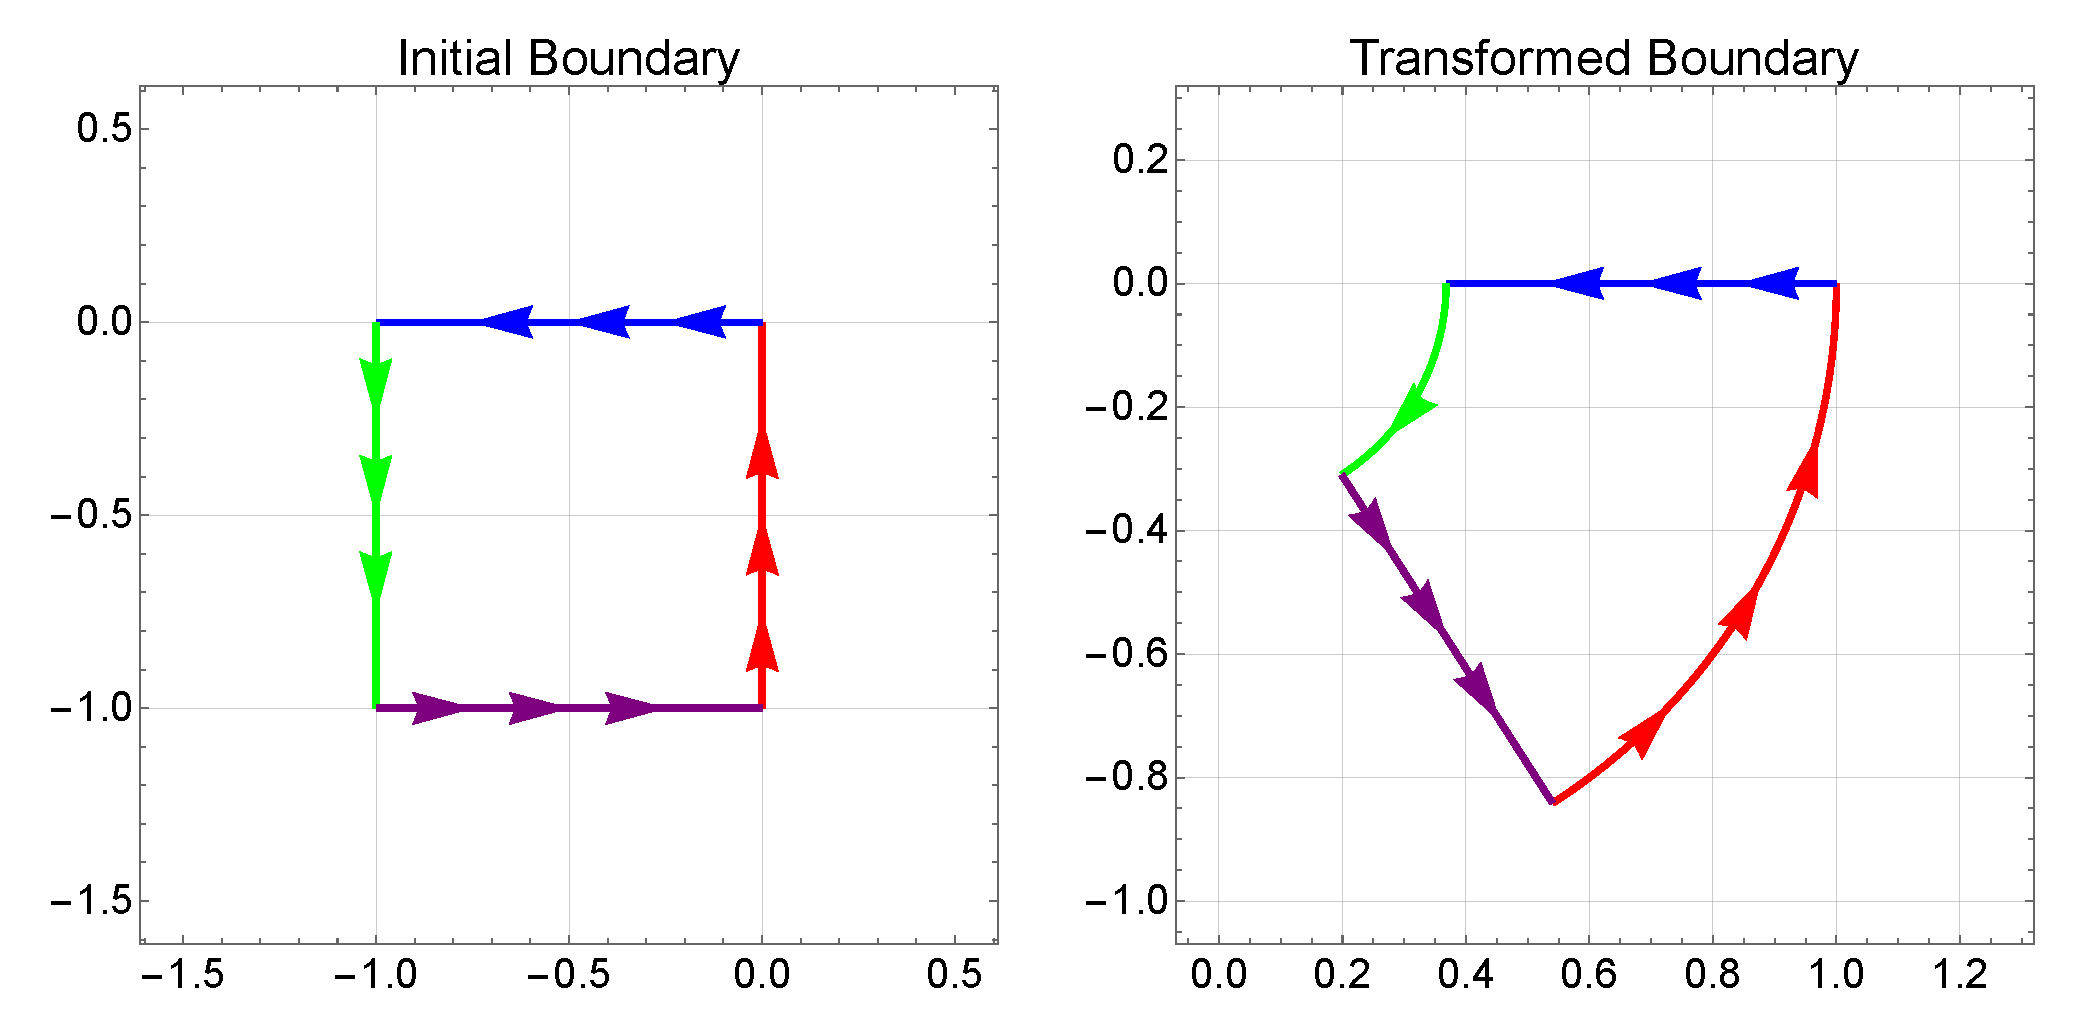
\includegraphics[width=0.85\textwidth]{images/hw_5/problem_2(1).pdf}
    \caption{Границя $\partial\omega(\mathcal{D})$. Різними кольорами відмічено різні сторони квадрату.}
    \label{fig:2(1)}
\end{figure}

\begin{figure}
    \centering
    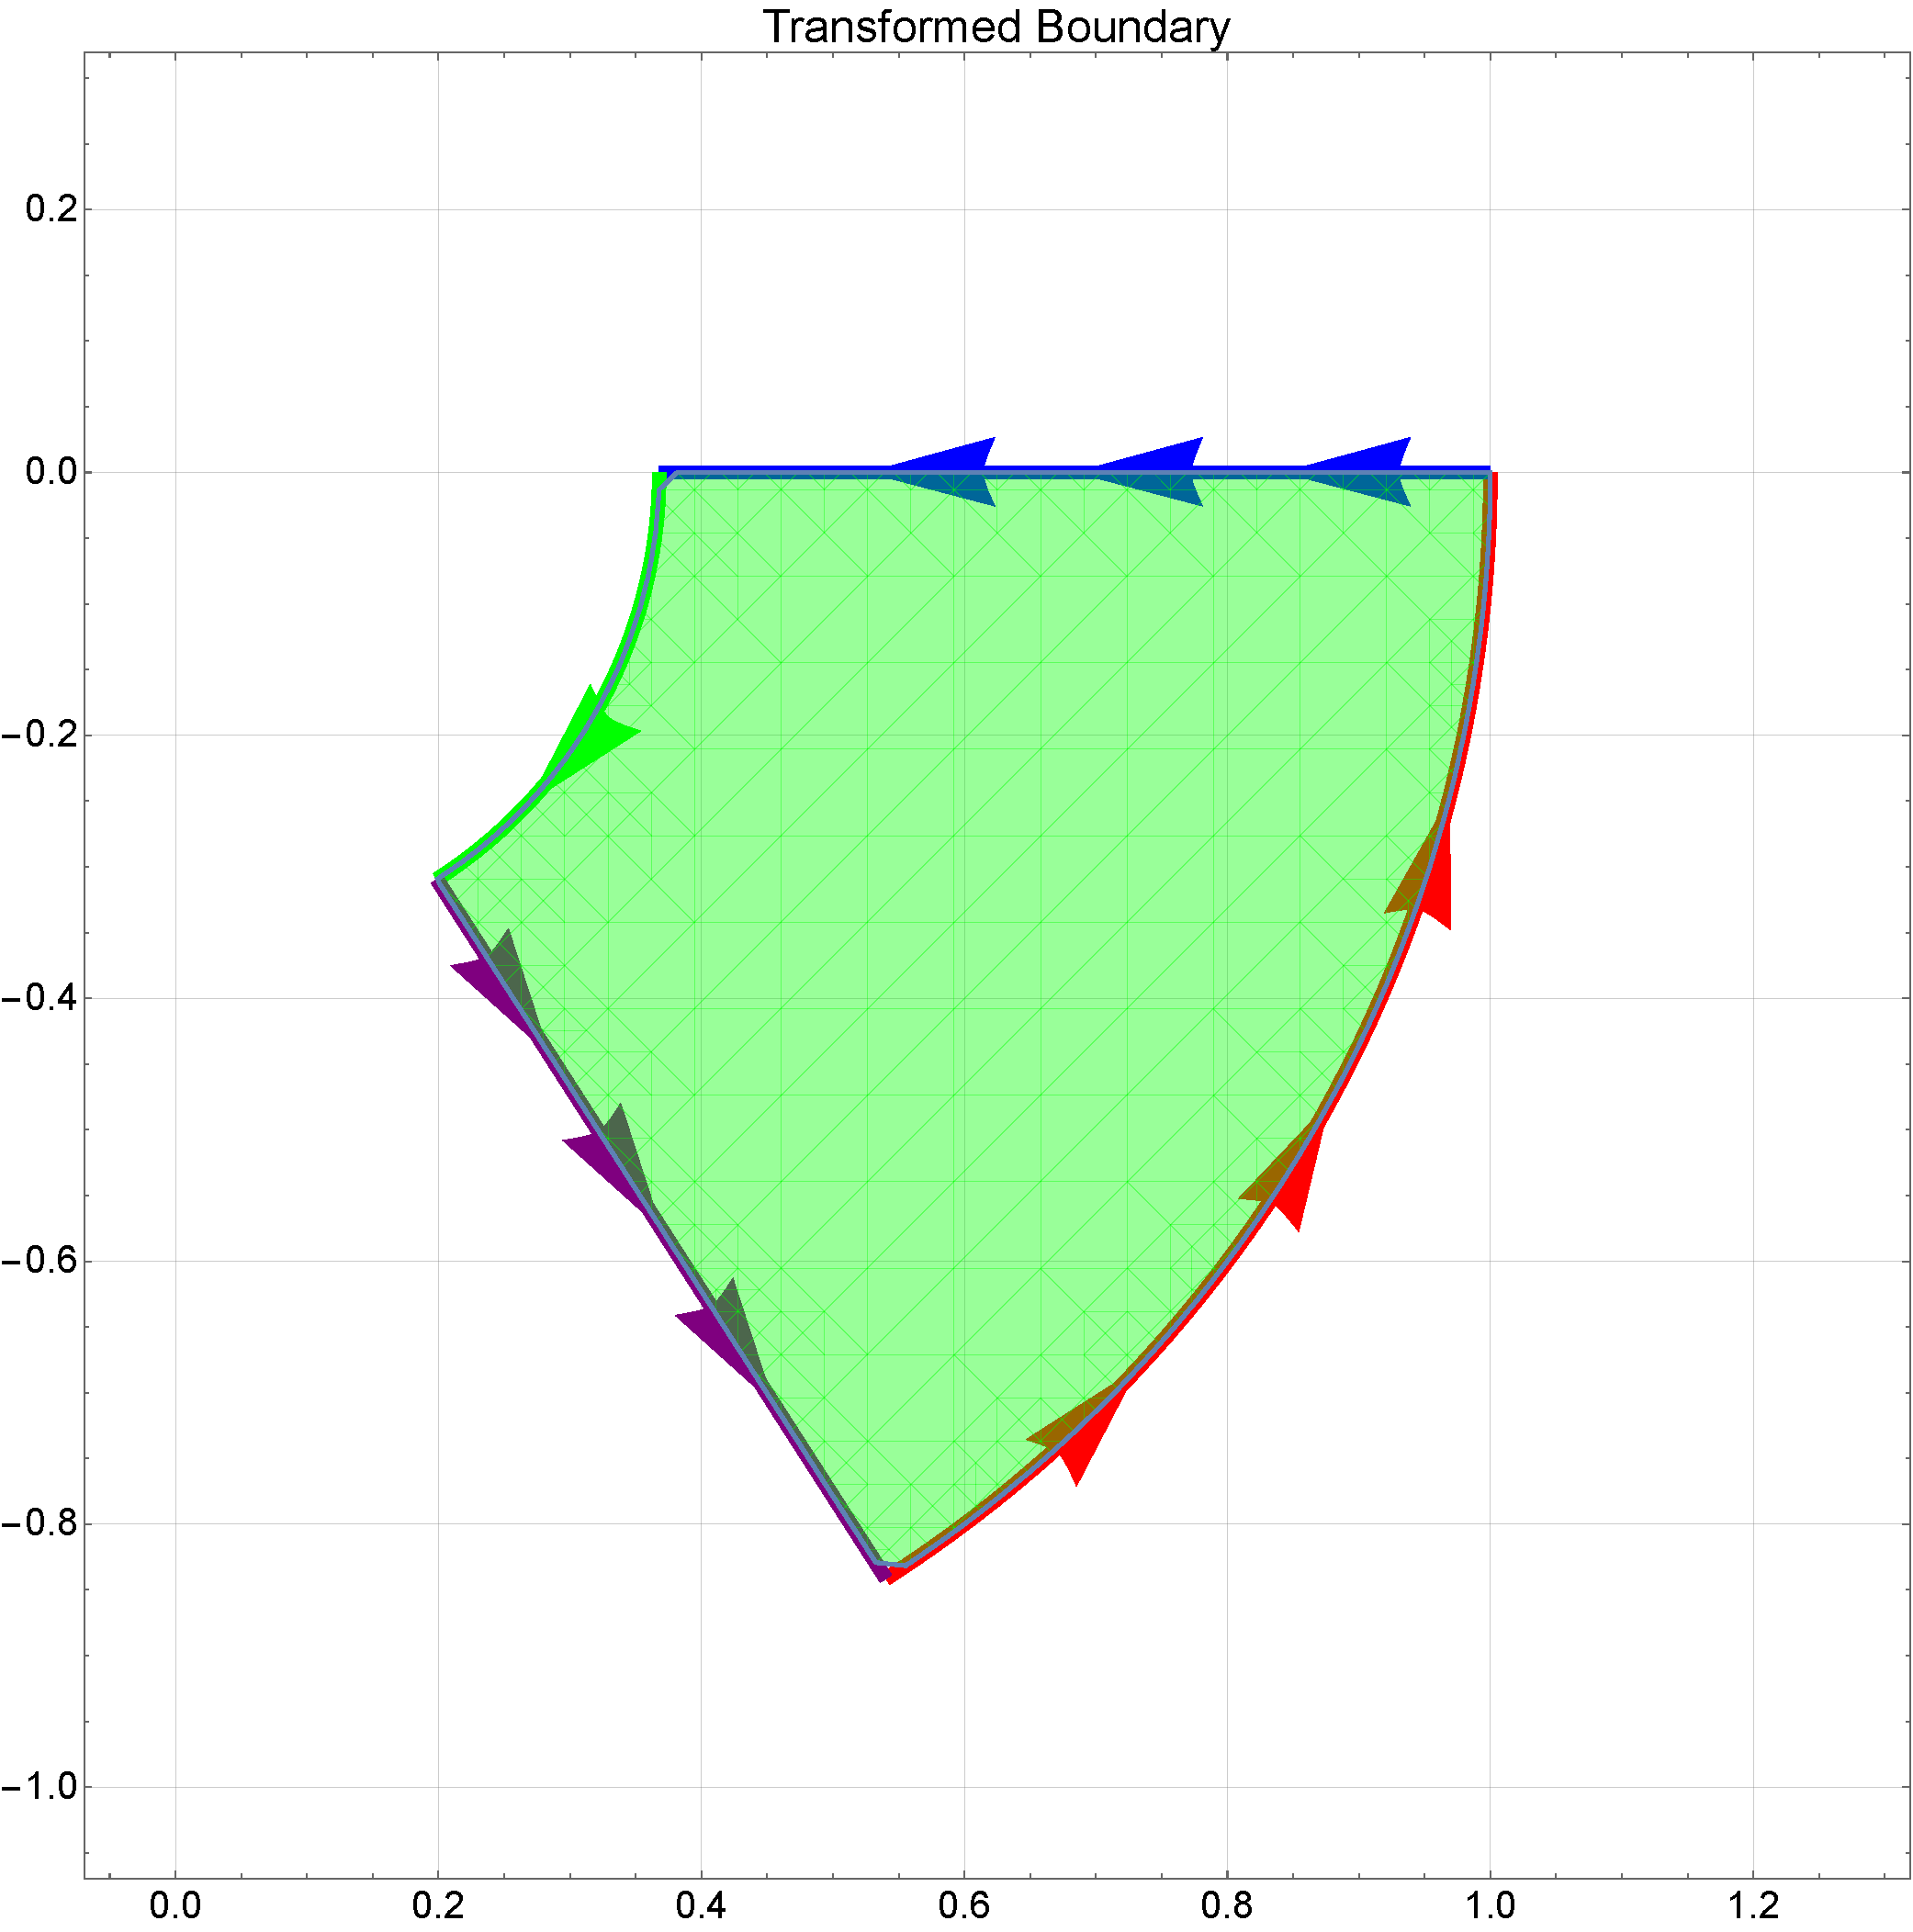
\includegraphics[width=0.8\textwidth]{images/hw_5/problem_2(2).pdf}
    \caption{Шуканий образ, відмічений зеленим.}
    \label{fig:2(2)}
\end{figure}

\problem{Придумати відображення}

\hspace{20px}\textbf{Умова.} Знайти функцію, яка здійснює конформне відображення області на верхню напівплощину $\text{Im}(z) > 0$ (двома способами).
\begin{equation}
    \mathcal{D} = \{z \in \mathbb{C}: z \neq [-2, 5]\}
\end{equation}

\textbf{Розв'язок.}

\textbf{Спосіб 1.} Ідейно: спочатку перетворимо $\mathcal{D}$ на множину $z \neq (0,+\infty)$, а далі перетворенням $z \mapsto \sqrt{z}$ завершимо все.

Отже, шукаємо таке лінійне-дробове перетворення, що зробить наступні відповідності: $-2 \mapsto 0, 5 \mapsto +\infty$. В якості такого перетворення візьмемо $\omega_1(z) := \frac{z+2}{5-z}$. Далі застосувавши перетворення $\omega_2(z) := \sqrt{z}$ переведемо $z \neq (0,+\infty)$ у множину $\text{Im}(z) > 0$. Отже, $\omega(z) = \omega_2 \circ \omega_1(z) = \sqrt{\frac{z+2}{5-z}}$. Весь процес зображено на Рисунку \ref{fig:3(1)}.

\begin{figure}
    \centering
    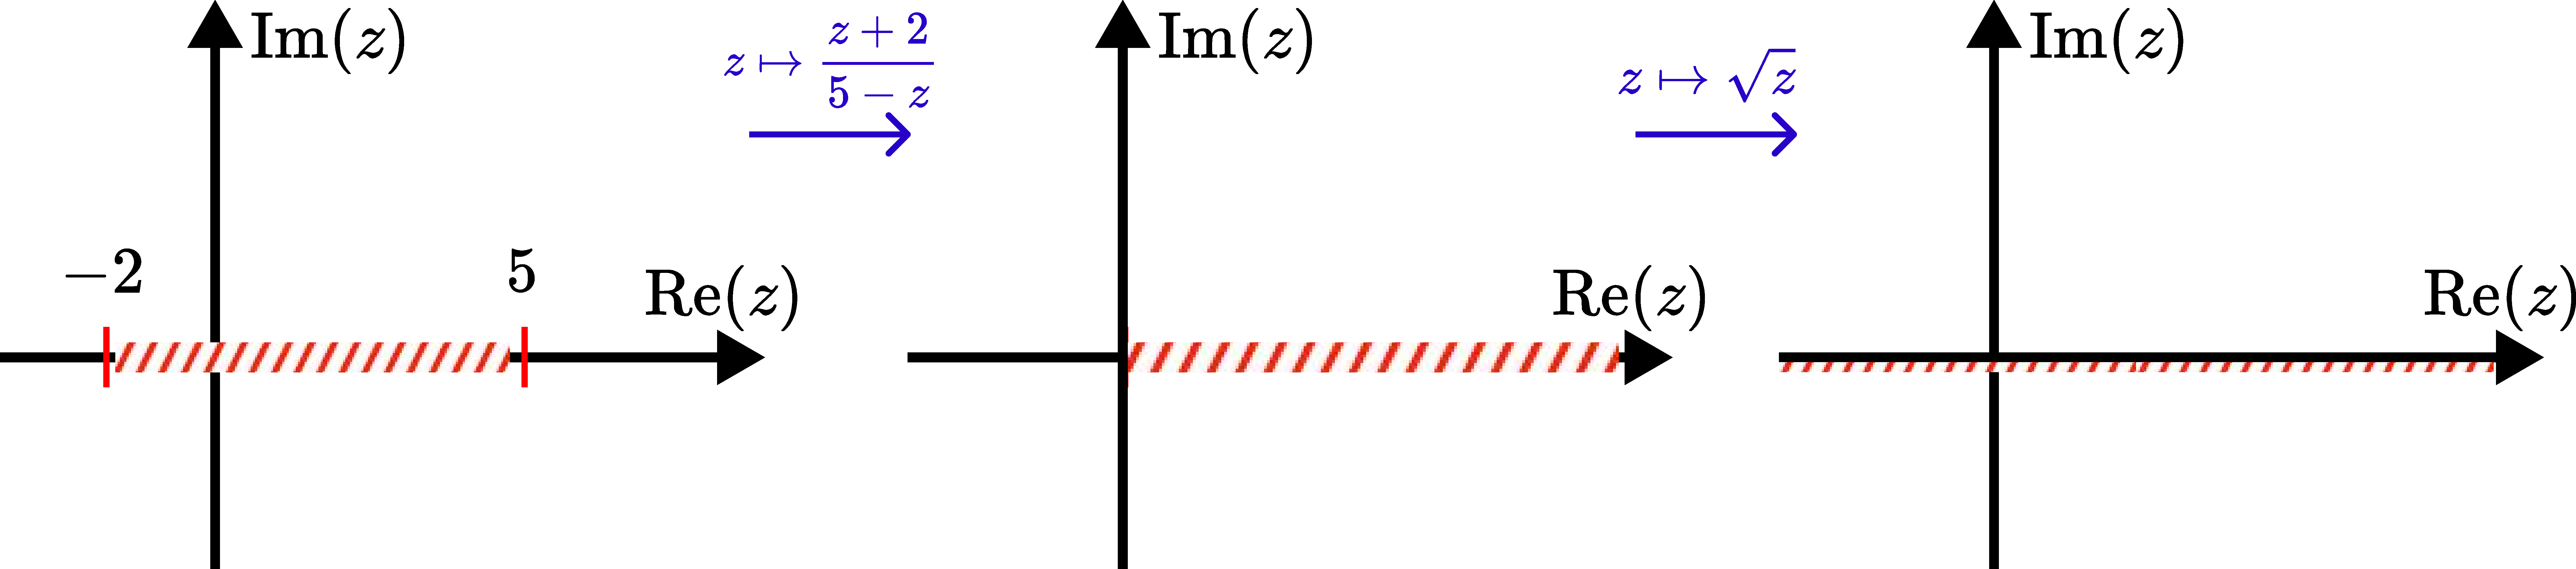
\includegraphics[width=\textwidth]{images/hw_5/problem_3(1).pdf}
    \caption{Серія перетворень, спосіб 1.}
    \label{fig:3(1)}
\end{figure}

\textbf{Спосіб 2.} Ідейно: переводимо спочатку $\mathcal{D}$ у відрізок $z\neq[-1,1]$, далі у $z \neq \mathbb{R} \setminus [-1,1]$, а після цього застосуємо обернену функцію Жуковського.

Отже, спочатку зведемо $z\neq[-2,5]$ у $z \neq [-1,1]$. Для цього, наприклад, застосуємо лінійне перетворення $\omega_1(z) = \frac{2}{7}\left(z-\frac{3}{2}\right)=\frac{2z-3}{7}$ -- легко побачити, що ми при цьому відобразимо $-2 \mapsto -1, 5 \mapsto 1$. 

Далі, застосуємо відображення $\omega_2(z) = \frac{1}{z}$, що відобразить $z \neq [-1,1]$ на $z \neq \mathbb{R}\setminus [-1,1]$. Далі залишається лише застосувати обернену функцію Жуковського $\omega_3(z) = z+\sqrt{z^2-1}$, що перетворить все на шукану напівплощину $\text{Im}(z)>0$. Весь процес зображено на Рисунку \ref{fig:3(2)}. Компануємо все у купу:
\begin{equation}
    \omega(z) = \omega_3 \circ \omega_2 \circ \omega_1(z) = \omega_3\left(\frac{7}{2z-3}\right) = \frac{7}{2z-3} + \sqrt{\left(\frac{7}{2z-3}\right)^2-1}
\end{equation}

\begin{figure}
    \centering
    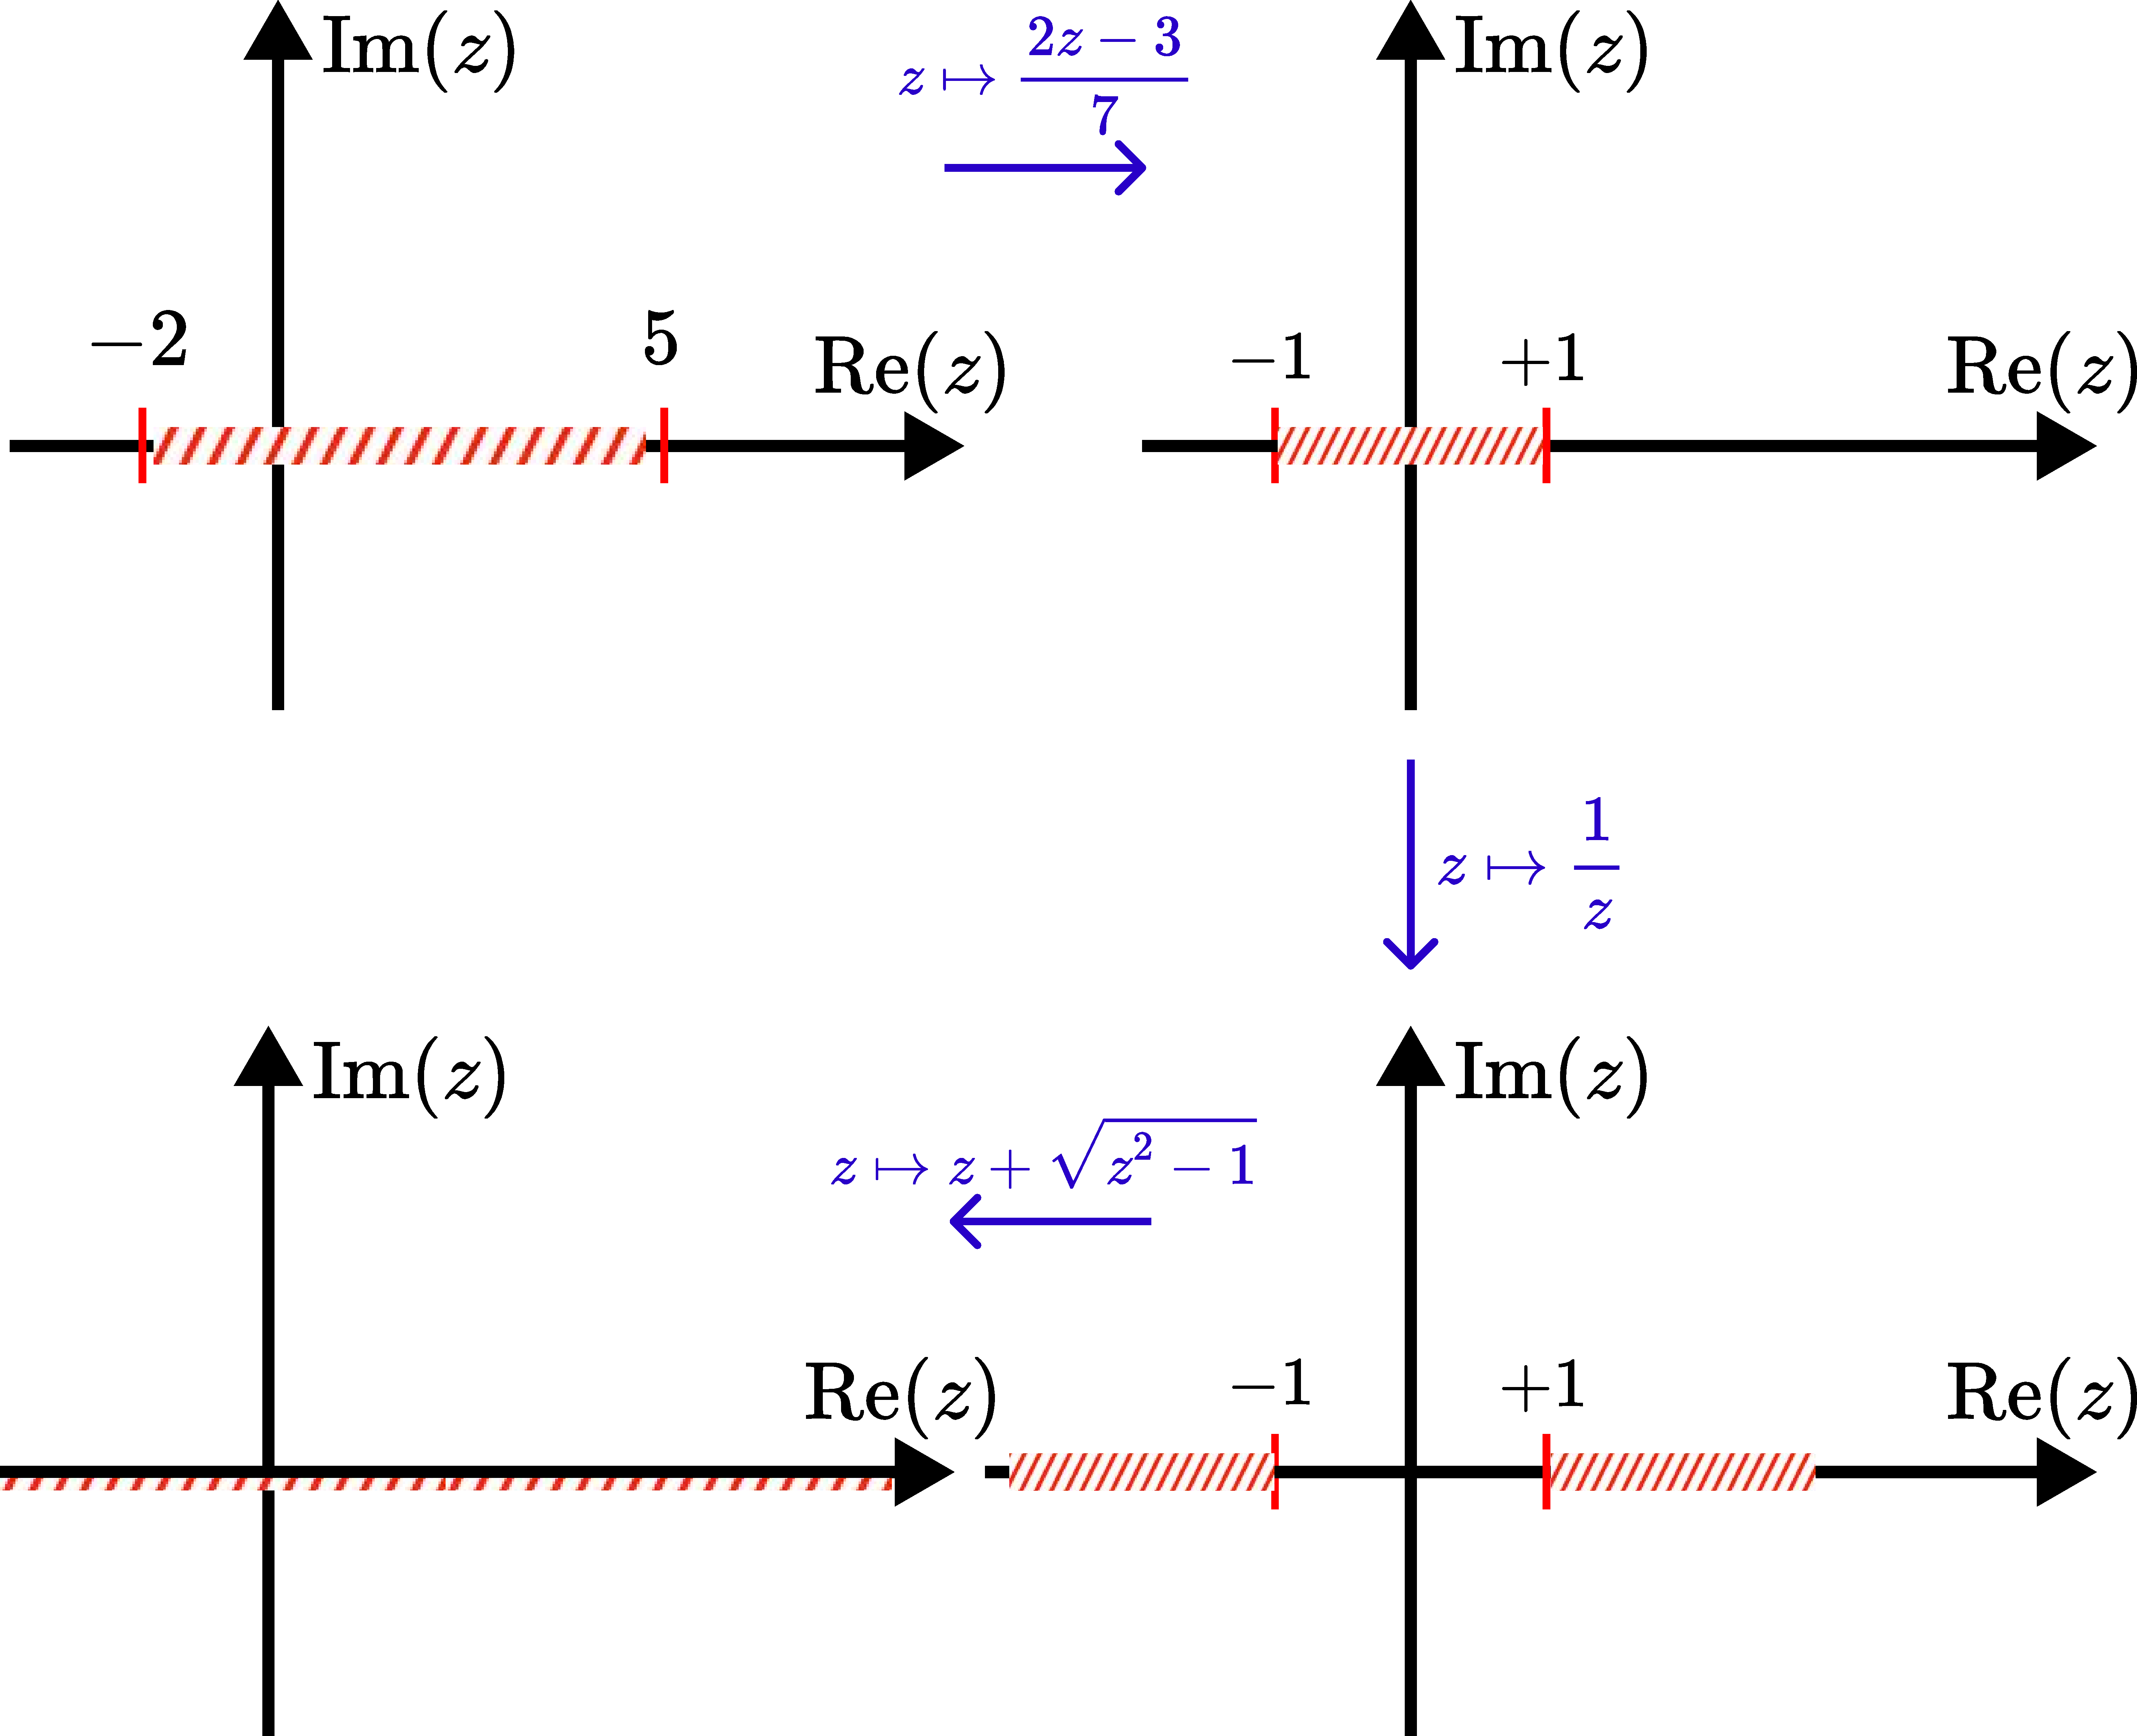
\includegraphics[width=\textwidth]{images/hw_5/problem_3(2).pdf}
    \caption{Серія перетворень, спосіб 2}
    \label{fig:3(2)}
\end{figure}

\textbf{Відповідь.} Або $\omega(z) = \sqrt{\frac{z+2}{5-z}}$, або $\omega(z) = \frac{7}{2z-3} + \sqrt{\frac{49}{(2z-3)^2}-1}$.

\end{document}
